\documentclass[dvipdfmx]{jsarticle}
\usepackage{graphicx}
\usepackage{url}
\usepackage{graphics}

\title{ソフトウェア設計及び実験\\前期・個人開発企画書\\
    \huge{そ〜だっしゅ！}
}
\author{学生番号 \ 6125010806　氏名 \ 清水 \ 統貴}
\date{2026年6月24日提出}

\begin{document}
\maketitle

\section{ゲーム内容}
%
\subsection{タイトル}
%
そ〜だっしゅ！

\subsection{ジャンル}
%
横スクロールアクションゲーム

\subsection{コンセプト・概要}
%
本ゲームはオリジナルキャラクターを操作してゴールを目指す横スクロール
アクションである.\\
最大の特徴はJoyConを振ることでたまる,\ 体力も兼任している「炭酸ゲージ」を使い,\ ブーストすることで
敵を倒しながらフィールド上を縦横無尽に高速飛行できるシステムである. 

\subsection{世界観}
%
かつてシュワシュワで平和だった「炭酸王国」が,\ 気の抜けた「ドロドロ帝国」によって
侵略されてしまった.\ プレイヤーは炭酸王国の勇者「ソーダマン」となり,\ 自らの炭酸
パワーを弾けさせ,\ 帝国軍をシュワっと浄化しながら駆け抜ける.\\

\subsection{ルール}
%
キャラクターを操作して,\ 5分以内にステージ右恥のゴール地点に到達すればクリアとなる.\ 道中で
敵やキャップを集めるとスコアが上がる.\ 時間切れ,\ 通常状態で敵に接触,\ ステージに配置された穴
に落ちる,\ 消費のしすぎ等で「炭酸ゲージ」が0になるととゲームオーバーとなる.\\

\subsection{UI}
%
\subsubsection{画面構成}
%
ウィンドウサイズは640×480とする.\\
\begin{itemize}
\item メイン画面：キャラクターと横スクロールの地形
\item UI表示：画面左上にペットボトル型の「炭酸ゲージ」,\ 画面右上にスコアとタイマー
を配置する
\end{itemize}

画面構成のイメージを図\ref{figure1}に示す.\\
\begin{figure}[htb]
    \centering
    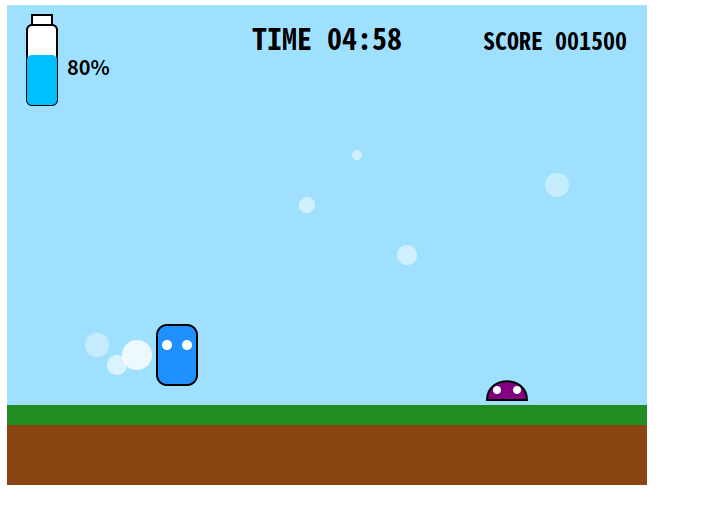
\includegraphics[scale=0.3]{gamenkousei.png}
    \caption{画面構成イメージ}
    \label{figure1}
\end{figure}

\subsubsection{操作方法}
%
操作はJoyCon,\ PROコントローラー,\ キーボードを使い,\ 下記に従う.\\
\begin{tabular}{l|l}
    命令 & 内容 \\ \hline
    移動 & アナログスティックまたは十字キーで左右移動. ゲージ使用時は全方向へ移動\\
    ジャンプ & コントローラー使用時は右ボタン, キーボード使用時はspaceキー\\
    ゲージの蓄積 & Joy-Con, Proコントローラーを上下に振る, キーボード使用時はWキーを連打\\
    ゲージの使用, 解除 & コントローラーの左ボタン, キーボード使用時は左シフトキー\\
\end{tabular}

\section{実装方法}
%
実装にはSDLを用いる,\ SDLについては,\ 授業資料を参考にする.\\

\subsection{利用デバイス}
%
Joy-Con,\ Proコントローラー,\ キーボードを用いる.\ なお,\ Joy-ConまたはProコントローラー
推奨である.\\

\subsection{データ構造}
%
現時点で必要だと考えられる変数,\ 構造体を示す(表\ref{table1-1}) \ (表\ref{table1-2})
\begin{table}[htb]
    \begin{center}
        \caption{データ構造(共通)}
        \label{table1-1}
        \begin{tabular}{|c||c|l|}\hline
            \multicolumn{3}{|l|}{共通の構造}\\ \hline
            データ型 & 変数名 &  \\ \hline \hline
            int & type & オブジェクトの型（キャラ,\ アイテム,\ エフェクト等） \\ \hline
            unsigned short & id & オブジェクトの識別番号 \\ \hline
            SDL\_Point & pos & オブジェクトの座標(x,\ y) \\ \hline
            int & depth & 描画の優先度(深さ) \\ \hline
        \end{tabular}
    \end{center}
\end{table}

\begin{table}[htb]
    \begin{center}
        \caption{データ構造(プレイヤー固有)}
        \label{table1-2}
        \begin{tabular}{|c||c|c|}\hline
            \multicolumn{3}{|l|}{キャラ固有の構造}\\ \hline
            データ型 & 変数名 &  \\ \hline \hline
            int & gauge & 炭酸ゲージの蓄積量(0〜100) \\ \hline
            int & state & 現在の状態(0：通常時,\ 1：ブースト中) \\ \hline
            unsigned int & score & 獲得スコア \\ \hline
            Uint32 & \verb+start_time+ & ステージ開始時のシステム時刻(\verb+SDL_GetTicks+等で取得)\\ \hline
            int & \verb+time_left+ & 残り時間(秒).\ 0になったらgaugeを0にして終了\\ \hline
        \end{tabular}
    \end{center}
\end{table}

\subsection{モジュール}
%
現時点で必要だと考えられる関数をモジュールごとに示す（表\ref{table2-1}）．

\noindent
(1)ユーザインタフェイス(gui\_process.c)
\par

\begin{table}[htb]
    \begin{center}
        \caption{ユーザインタフェイス関係関数}
        \label{table2-1}
        \begin{tabular}{|c||l|}\hline
            \multicolumn{2}{|l|}{\bf{void InitWindows(void)}}\\ \hline
            関数名 & InitWindows()  \\ \hline \hline
            機能 & ウィンドウの初期化処理を行う関数 \\
            引数 & なし \\
            返り値 & なし \\ \hline
            \multicolumn{2}{|l|}{\bf{Bool WindowEvent(void)}}\\ \hline
            関数名 & WindowEvent()  \\ \hline \hline
            機能 & イベントを取得し，処理する関数 \\
            引数 & なし \\
            返り値 & 終了フラグ（True：処理継続，False：終了） \\ \hline
        \end{tabular}
    \end{center}
\end{table}

(2)各モジュールの外部関数
    \begin{table}[htb]
        \begin{center}
            \caption{外部関数}
            \label{table2-2}
            \resizebox{\textwidth}{!}{
                \begin{tabular}{|c||c|c|c|}\hline
                    \multicolumn{4}{|l|}{モジュールの外部関数}\\ \hline
                    関数名 & 機能 & 引数 & 返り値 \\ \hline \hline
                    InitSystem & ウィンドウとSDL,\ Joy-Conセンサーの初期化 & なし & 成功/失敗フラグ\\ \hline
                    UpdateInput() & Joy-Conのセンサー値と\ ボタン入力の取得 & なし & 入力データ構造\\ \hline
                    UpdatePhysics() & 重力処理,\ 地形・敵との当たり判定\ (コリジョン)の計算 & プレイヤー構造体へのポインタ & なし\\ \hline
                    DrawGraphyics() & スプライト画像と\ UIの画面描画 & 描画対象のリスト & なし\\ \hline
                \end{tabular}
            }
        \end{center}
    \end{table}

\section{ガントチャート}
%
図\ref{figure2}のようにガントチャートを作成した.\\
\begin{figure}[htb]
    \centering
    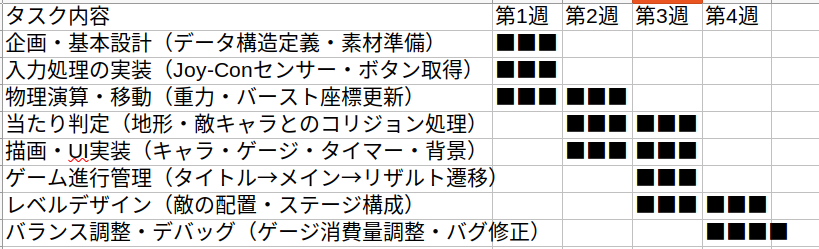
\includegraphics[scale=0.3]{ganttchart.png}
    \caption{ガントチャート}
    \label{figure2}
\end{figure}

\section{自己評価と理由}
%
表\ref{table3}に示すように,\ すべて2点の合計6点で,\ 合格基準を満たしていると考える.\\

\begin{table}[htb]
    \begin{center}
        \caption{自己評価と理由}
        \label{table3}
        \resizebox{\textwidth}{!}{
            \begin{tabular}{|c|c|l|}\hline
                項目 & 評価値 & 理由\\ \hline\hline
                ハードウェア構成 & 2 & Joy-Conの加速度センサーを利用し,\ 「振る」動作をゲーム進行に不可欠なゲージ蓄積の入力として実装する\\ \hline
                技術面 & 2 & センサー入力値のリアルタイムなスムージング処理と,\ 横スクロールアクションにおける重力・当たり判定（物理演算）を実装する\\ \hline
                独創性 & 2 & 独自にデザインしたキャラクターのグラフィックとタイトルロゴを使用する.\ 「振って力を溜め,\ 一気に解放する」という独自のアクション性を提供する\\ \hline
            \end{tabular}
        }
    \end{center}
\end{table}

\section{参考にしたゲーム}
%
スーパーマリオブラザーズを参考にした横スクロールアクションゲームを土台に,\ 固有のシステムを追加した.\\

\section{ゲームのアピールポイント}
%
本ゲームのアピールポイントは以下の通りである.\\

\begin{itemize}
\item フィジカルと連携した爽快感：コントローラーを振って力をため,\ 一気に開放する直感的なアクション
\item 戦略的なリソース管理：炭酸ゲージ＝体力＝必殺技のエネルギー」という仕様により,\ バーストの使いすぎが自爆を招くハイリスク・ハイリターンの駆け引き
\item 高いリプレイ性：5分という短い制限時間の中でクリアを目指す,\ テンポの良いゲームサイクル
\end{itemize}

\begin{thebibliography}{99}
%
% \bibitem{chatGPT} Open AI : ChatGPT \url{https://chatgpt.com/ja-JP} (2026年4月30日閲覧).
% %
% \bibitem{claude} Anthropic : Claude \url{https://claude.ai/new} (2026年5月5日閲覧).
% %
\bibitem{gemini} Google : Gemini \url{https://gemini.google.com/?hl=ja}
%

\end{thebibliography}
\end{document}